W poniższej pracy dokonamy analizy ruchu fotonów w pobliżu czarnej dziury, której promień Schwarzschilda wynosi $r_s=1$. Aby dodatkowo ułatwić rozważania, przyjmujemy $c=G=1$ i konsekwentnie $M=\frac{1}{2}$ oraz ustalamy $\theta=\frac{\pi}{2}$. Dodatkowo, wyliczymy symbole Christoffela drugiego rodzaju dla metryki Schwarzschilda.

\subsection{Symbole Christoffela}

Dla wygody, nie będziemy wyliczać symboli Christoffela wprost z definicji. Zamiast tego, skorzystamy z lagrangianu, który spełnia równanie
%/*Oczywiście, wyliczyć symbole Christoffela można wprost z ich definicji. Prostsze jest jednak użycie lagrangianu, który spełnia*/
$$ S = \int L d \lambda, $$
gdzie $\lambda$ jest afiniczną parametryzacją, a $S$ to działanie, czyli w prostym przypadku cząsteczki poruszającej się wzdłuż pojedynczej krzywej jest to suma iloczynu pędu cząsteczki z fragmentem drogi przebytej \cite{mechanics}. 

%//Używając więc tych faktów w przypadku fotona poruszającego się w metryce Schwarzschilda dostajemy
Stosując więc powyższe wiadomości dla przypadku fotonu poruszającego się w metryce Schwarzschilda dostajemy
$$ S = \int d \tau= \int \frac{d \tau}{d \tau} d \tau = \int \frac{\sqrt{d \tau^2}}{d \tau} d \tau = \int \sqrt{g_{\mu, \nu}\dot{x^\mu} \dot{x^\nu}}d \tau = \int L' d \tau. $$
W takim razie jednym z interesujących nas lagrangianów jest 
$$L'=\sqrt{g_{\mu, \nu}\dot{x^\mu}\dot{x^\nu}}.$$ 
Ponieważ lagrangian nie jest unikalny, i nałożenie na niego dowolnej funkcji dalej daje lagrangian, to możemy wybrać
$$L=(L')^2 = g_{\mu,\nu}\dot{x^\mu}\dot{x^\nu}.$$
Ułatwi to nam wyliczenia korzystające z drugiego równania lagrangianu, to znaczy:
$$\frac{d}{ d \tau}\left(\frac{\partial L}{\partial \dot{x^\mu}}\right)= \frac{\partial L}{\partial x^\mu}\; (\text{patrz \cite{mechanics}}). $$
Podstawiając do $d \tau$ metrykę Schwarzschilda dostajemy poniższy układ równań:

\begin{align*}
  \ddot{t}&=-\frac{1}{r(r-1)}\dot{r}\dot{t}\\
  \ddot{r}&=-\frac{r-1}{ 2r^3} \dot{t}^2+\frac{1}{2r(r-1)}\dot{r}^2+(r-1)\dot{\theta}^2+(r-1)\sin^2\theta \dot{\phi}^2\\
  \ddot{\theta} &= \sin \theta \cos \theta \dot{\phi}^2 - \frac{2}{ r} \dot{r}\dot{\theta}\\
  \ddot{\phi} &= -\frac{2}{r} \dot{r}\dot{\phi} - 2 \frac{\cos \theta}{ \sin \theta} \dot{\phi}  \dot{\theta} 
\end{align*}
Zauważmy, że otrzymane wyżej równania to tak naprawdę geodezyjna w metryce Schwarzschilda. Z lewej strony równości można więc z łatwością sczytać symbole Christoffela - są to współczynniki przy odpowiednich pochodnych. Ponieważ interesuje nas tylko ruch fotonów po płaszczyźnie $\theta=\frac{\pi}{2}$, to $\dot{\theta}=0$, $\cos \theta=0$ i $\sin \theta=1$.

Symbole Christoffela w interesującym nas przypadku są więc równe
\begin{align*}
  \Gamma_{t,r}^t&=\frac{1}{2r(r-1)}\\ 
  \Gamma_{t,t}^r&=\frac{r-1}{2r^3}\\ 
  \Gamma_{r,r}^r&=-\frac{1}{2r(r-1)}\\ 
  \Gamma_{\phi,\phi}^r&=-(r-1)\\ 
  \Gamma_{r,\phi}^\phi&=\frac{1}{r} 
\end{align*}

\subsection{Równanie orbity}

Korzystając jeszcze raz z drugiego równania lagrangianu, dostajemy
$$ \frac{d}{d\tau}(2r^2\dot{\phi})=0 $$
$$ \frac{d}{d\tau}\left(2\frac{r-1}{r}\dot{t}\right)=0 $$
czyli 
$$ r^2\dot{\phi}=a \implies \dot{\phi}=\frac{a}{r^2}$$
$$ \frac{r-1}{r}\dot{t}=\frac{a}{b} \implies \dot{t}=\frac{ra}{b(r-1)}$$
dla pewnych stałych $a,b$. Z fizycznego punktu widzenia $a$ będzie pędem kątowym cząsteczki, natomiast $\frac{a}{b}$ jest energią całkowitą.
%Dzieląc teraz równanie $\dot{t}$ przez równanie $\dot{r}$ uniezależniamy równanie wyżej od czasu właściwego $\tau$.
%$$ \frac{d t}{d\phi}=\frac{br^3}{a(r-1)}$$

%Przekształcając teraz wzór na metrykę Schwarzschilda dostajemy równanie uzależniające $r$ od $\phi$:
%\begin{align*}
%  1&=-\frac{r-1}{r}\dot{t}^2+\frac{r}{r-1}\dot{r}^2+r^2\dot{\phi}^2\\ 
%  \frac{r-1}{r}&=-\frac{(r-1)^2}{r^2}\dot{t}^2+\dot{r}^2+r(r-1)\dot{\phi}^2\\ 
%  %\dot{r}^2&=\frac{r-1}{r}+\frac{(r-1)^2}{r^2}\cdot \frac{a^2r^2}{b^2(r-1)^2}-r(r-1)\frac{a^2}{r^4}\\
%  \dot{r}^2&=\frac{r-1}{r}+\frac{a^2}{b^2}-\frac{a^2(r-1)}{r^3}\\
%  \left(\frac{d r}{d\phi}\right)^2&=\frac{(r-1)r^3}{a^2}+\frac{r^4}{b^2}-r(r-1)\\ 
%  \left(\frac{dr}{d\phi}\right)^2&=\frac{r^4}{b^2}+\frac{r-1}{r}\left(\frac{r^4}{a^2}-r^2\right)
%\end{align*}
%Jak już zostało wspomniane, 
%$$r^2\dot{\phi}^2=a=\frac{L}{\mu},$$
%gdzie $\mu$ to zredukowana masa układu, wynosząca
%$$\mu=\frac{mM}{m+M}=0,$$
%bo $M=1$, ale $m=0$ jako masa fotonu. W takim razie $a\to \infty$ jeśli będziemy zmniejszać masę cząsteczki do $0$. Dla pozostawienia $b$ jako stałej bez wyrazu $r$, wykonamy podstawienie
%$$\begin{matrix}u=\frac{1}{r}\\ -r^2du=dr\end{matrix}$$
%otrzymując ostatecznie równanie orbity
%$$\left(\frac{du}{d\phi}\right)^2=\frac{1}{b^2}+(1-u)\left(\frac{1}{a^2}-u^2\right)\xrightarrow{a\to\infty}\frac{1}{b^2}-u^2(1-u)$$
%które możemy obustronnie zróżniczkować względem $\phi$ by otrzymać
%$$2u''u'=3u^2\cdot u'-2u\cdot u'$$
%$$u''=u\left(\frac{3}{2}u-1\right)$$
%z czego od razu widać, że orbitą stałą jest 
%$$u=\frac{2}{3}\implies r=\frac{3}{2}$$
%

Możemy teraz wyznaczyć $t$ w zależności od $\phi$, pozbywając się zależności od $\tau$:
$$\frac{dt}{d\phi}=\frac{r^3}{b(r-1)}$$
Przekształcając teraz drugi warunek geodezyjnej \emph{nullowej}, dostajemy
\begin{align*}
  0&=-\frac{(r-1)^2}{r^2}(dt)^2+(dr)^2+r(r-1)(d\phi)^2\\ 
  (dr)^2&=\frac{(r-1)^2}{r^2}(dt)^2-r(r-1)(d\phi)^2\\ 
  \left(\frac{dr}{d\phi}\right)^2&=\frac{(r-1)^2}{r^2}\left(\frac{dt}{d\phi}\right)^2-r(r-1)\\ 
  \left(\frac{dr}{d\phi}\right)^2&=\frac{(r-1)^2}{r^2}\cdot\frac{r^6}{b^2(r-1)^2}-r(r-1)\\ 
  \left(\frac{dr}{d\phi}\right)^2&=\frac{r^4}{b^2}-r(r-1)
\end{align*}
a stosując podstawienie 
$$u=\frac{1}{r},\quad -r^2du=dr$$
wyraz $\frac{1}{b^2}$ stanie się wyrazem wolnym, znikającym po różniczkowaniu względem $\phi$:
\begin{align}
  \left(\frac{du}{d\phi}\right)^2&=\frac{1}{b^2}-u^2+u^3\label{rownanie_orbity}\\ 
  u'' &=u\left(\frac{3}{2}u-1\right)\label{zmiana predkosci}
\end{align}

\renewcommand{\figurename}{Wykres}
\begin{figure}[h]
  \centering
  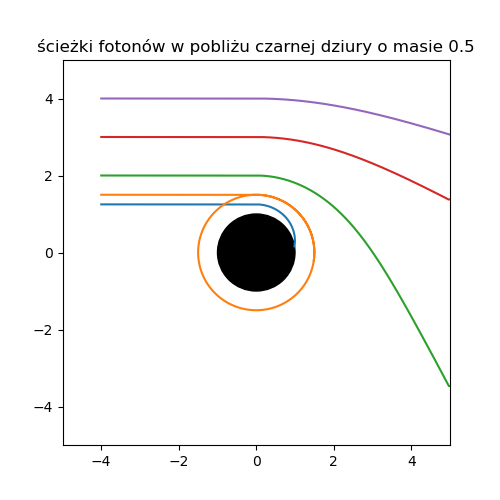
\includegraphics[width=0.8\textwidth]{ilustracje/sceizki_wykres.png}
  \caption{Ścieżki fotonów w pobliżu czarnej dziury o masie $M=\frac{1}{2}$ i promieniu Schwarzschilda $r_s=1$ ($c=1=G$) uzyskane przy pomocy języka Python.}\label{wykres fotonow}
\end{figure}

Powyższe równanie \ref{zmiana predkosci} w jasny sposób pokazuje, że orbita stacjonarna w przypadku czarnej dziury o promieniu Schwarzschilda $1$ pojawia się dla $r=\frac{3}{2}$. Wspomniana orbita została zaznaczona na wykresie \ref{wykres fotonow}, który prezentuje również rozmiar czarnej dziury (czarne koło pośrodku). Równanie \ref{zmiana predkosci} zostało rozwiązane przy pomocy funkcji \verb+odeint+ z biblioteki \verb+scipy+ języka Python i trajektorie pięciu fotonów, z czego część nie zapada się w czarną dziurę, zostały pokazane na wykresie \ref{wykres fotonow}





%/* 
%Oczywiście, $accent(r, diaer)=0$, bo foton nie przyśpiesza. Możemy więc podzielić drugie równanie przez $accent(phi, dot)^2$, by dostać:
%
%$ 0=frac(r-1, 2r^3)(frac(accent(t, dot), accent(phi, dot)))^2 +frac(1, 2r(r-1))(frac(accent(r, dot), accent(phi, dot)))^2 - (r-1) $
%$ (frac(accent(r, dot), accent(phi, dot)))^2=2r(r-1)^2-frac((r-1)^2, r^2)(frac(accent(t, dot), accent(phi, dot)))^2. $
%
%*/
%
%Chcemy teraz wydobyć $\dot{t}$ oraz $\dot{\phi}$ - wtedy będziemy wiedzieli jak wyrazić $\frac{\dot{t}}{\dot{\phi}}$. Wracając do drugiej równości lagrangiana wykorzystanej dla $phi$ oraz $t$, dostaniemy:
%$ 
%  frac(d, d tau) (2r^2 accent(phi, dot))&=0\ 
%    frac(d, d tau) (2frac(r-1, r)accent(t, dot))&=0
%$
%Co znaczy, że
%$ r^2 accent(phi, dot)=a => accent(phi, dot)=frac(a, r^2) $
%$ frac(r-1, r)accent(t, dot)=frac(a, b) => accent(t, dot) = frac(a r, b(r-1)) $
%dla pewnych stałych $a, b$.
%
%Przekształcając teraz metrykę Schwarzschilda, dostajemy
%$ frac(r-1, r) = frac((r-1)^2, r^2)accent(t, dot)^2 - accent(r, dot)^2 -r(r-1) accent(phi, dot)^2 $
%a podstawiając wartości $accent(phi, dot)^2$ i $accent(t, dot)^2$ wyliczone wyżej
%$ frac(r-1, r) = frac(a^2, b^2) - accent(r, dot)^2 - r(r-1)a^2 $
%$ accent(r, dot)^2 = frac(a^2, b^2) - frac(r-1, r)(1 + frac(a^2, r^2)). $
%Aby teraz wyliczyć równanie orbity, chcemy podzielić powyższe równanie przez $accent(phi, dot)^2=frac(a, r^2)$:
%$ ( frac(accent(r, dot), accent(phi, dot)) )^2 = frac(r^4, b^2) - frac((r-1), r)(frac(r^4, a^2)+r^2) $
%Trzeba tutaj zaznaczyć, że równanie wyliczone wyżej nie jest jeszcze krzywą geodezyjną po której podróżuje światlo - w przypadku wyżej wzięliśmy
%$ -1 = g_(mu, nu)accent(x^mu, dot)accent(x^nu, dot) $
%zamiast przyrównywać to do zera. Badamy więc chwilowo trasę cząsteczki z masą. Aby przejść do badania fotonu, chcemy aby $a arrow oo$. Fizycznie wartość ta jest tak naprawdę równa pędowi kątowemu $L$ wydzielonemu przez zredukowaną masę $mu$, tzn.
%$ r^2 accent(phi, dot)^2 = a = frac(L, mu) $
%a ponieważ zredukowana masa jest zależna od masy fotonu $m_1=0$, 
%$ mu = frac(m_1 m_2, m_1 + m_2), $
%gdzie $m_1, m_2$ to masy składowe układu dwóch ciał, to dla fotonu $mu=0$ i co za tym idzie, $a arrow oo$.
%
%\subsection{Równanie orbity}
%
%W równaniu orbity wyliczonym w poprzednim rozdziale zastosujemy podstawienie $u=frac(1, r)$, wtedy
%$ -r^2 accent(u, dot) = accent(r, dot). $
%Po takim podstawieniu równanie orbity to
%$ ( frac(accent(u, dot), accent(phi, dot)) )^2 = frac(1, b^2) - (1-u)(frac(1, a^2)+u^2) = frac(1, b^2)-(1-u)u^2 $
%bo jak wcześniej uzasadniliśmy, $a arrow oo$.
%
%Rozwiązanie powyższego równania dałoby zależność między $r$ a $phi$, bo możemy usunąć trzymaną z tyłu głowy informację o $tau$:
%$ (frac(d u, d phi))^2 = frac(1, b^2) -(1-u)u^2. $
%Bez trudu wyciągniemy też informację o drugiej pochodnej $u$:
%$ 2u'(phi)u''(phi) = -2u + 3u^2 $
%$ u''(phi) = -u + frac(3, 2) u^2=u(frac(3, 2)u-1), $
%bo $u'=c=1$ w naszym układzie. Stąd widać, że $u=0$ oraz 
%$ frac(2, 3)=u=frac(1, r) => r = frac(3, 2) $ 
%są punktami przegięcia funkcji $u(phi)$. Dalej, dla 
%$ frac(2, 3)< u = frac(1, r) => r < frac(3, 2) $ 
%pochodna $u'(phi)$ powinna być rosnąca (czyli $r'=-r^2u'$ maleje), a dla 
%$ frac(2, 3) > u=frac(1, r) => r > frac(3, 2) $ 
%powinna być malejąca ($r'=-r^2u'$ rośnie).
%
%Możemy więc obserwować pierwiastki powyższej równości, by sprawdzać, kiedy $r(phi)$ jest stałe. Co więcej, możemy również sprawdzić przy jakim położeniu foton zapadnie się w czarną dziurę, a kiedy będzie w stanie uciec z jej pobliża.
%
%Równanie wyżej jest równaniem 3 stopnia o rzeczywistych współczynnikach, ma więc ono 3 pierwiastki, co najmniej jeden rzeczywisty i dwa potencjalnie zespolone, sprzężone ze sobą. Możemy oznaczyć je przez $u_1, u_2, u_3$ i zapisać
%$ 
%  (frac(d u, d phi))^2 &= (u- u_1) (u- u_2) (u-u_3)= \
%    &= u^3 - u^2 (u_1 + u_2 + u_3)+ \ 
%      &+ u(u_1 u_2 + u_1 u_3 + u_2 u_3) +\ 
%        &-u_1 u_2 u_3. 
%$
%
%Widzimy więc, że suma pierwiastków odpowiada wyrazowi przy $u^2$ w oryginalnym równaniu, natomiast ich iloczyn jest równy wyrazowi wolnemu:
%$ 
%  u_1 + u_2 + u_3 = 1
%$
%$
%  -frac(1, b^2) = u_1 u_2 u_3
%$
%%/* 
%%Warto też zauważyć, że oryginalne równanie nie posiada wyrazu stopnia $1$, czyli 
%%$ 0= u_1 u_2 + u_1 u_3 + u_2 u_3 $
%%*/
%
%Z tego wzoru możemy od razu wyliczyć wzór na drugą pochodną
%$ (u'(phi))^2 = (u-u_1)(u-u_2)(u-u_3) $
%$ u''(phi)u'(phi) = frac(1, 2)[(u-u_2)(u-u_3) + (u-u_1)(u-u_2) + (u-u_1)(u-u_3)] $
%gdzie możemy sprawdzać jej wartość w punktach ekstremalnych funkcji $u(phi)$.
%
%Zacznijmy od przypadku gdy $u_1 < u_2 < u_3$ są wszystkie liczbami rzeczywistymi. Wtedy dla $u_2 < u < u_3$ oraz $u < u_1$ funkcja $(u-u_1) (u-u_2) (u-u_3)$ jest ujemna, co daje zespoloną wartość dla $u'(phi)$. 
%
%Jeśli teraz $u_1$ będzie jedynym pierwiastkiem rzeczywistym, a $u_2$ i $u_3$ będą sprzężonymi ze sobą pierwiastkami zespolonymi. W takim przypadku jedyny pierwiastek rzeczywisty musi być ujemny, bo wtedy
%$ -frac(1, b^2) = u_1 u_2 u_3 = u_1 u_2 overline(u_2) = u_1 ("Re"(u_2)^2 + "Im"(u_2)^2) $
%gdzie $b^2$ oraz $"Re"(u_2)^2+"Im"(u_2)^2$ są zawsze dodatnimi wartościami.
%
%W takim razie $u_1$ będzie orbitą, z której fotony nie zapadają się, ale też nie mają szansy wypaść z okolic czarnej dziury. Z racji tego jak wyglądają czarne dziury, możemy z dużą dozą prawdy stwierdzić, że 
%$ u_1>r_s=1. $ 
%W takim razie $"Re"(u_2)="Re"(u_3)<0$.
%
